\begin{frame}
\frametitle{Microreactors: Motivation}
\begin{columns}
  \column[t]{5cm}
  Microreactors can fulfill energy needs in special use cases, or in
  areas with a greater population.
  \column[t]{5cm}
    \begin{figure}[htbp!]
    \begin{center}
    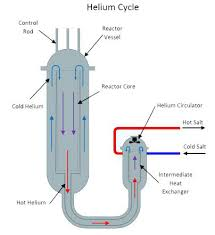
\includegraphics[height=4cm]{./images/mmr-chalk-river}
    \end{center}
    \caption{A Diagram of the proposed MMR for the Chalk River project. \cite{mmr-chalk-river}.}
    \label{fig:mmr-chalk-river}
    \end{figure}

\end{columns}
\end{frame}


\begin{frame}
\frametitle{Siting Considerations for Microreactors}

  \begin{itemize}
    \item Current guidelines based on LWRS
    \item Experience tells us radionuclide release is not as severe as once feared.
  \end{itemize}

  The first step in these revised siting considerations is to determine a source term.

\end{frame}
